\chapter{القوائم المتسلسلة (\textenglish{Linked lists})}

لكي نخزّن المعلومات في الذاكرة، استعملنا متغيّرات بسيطة (من نوع
\InlineCode{int}، \InlineCode{double} \dots)،
كما استعملنا جداول و هياكل مخصّصة. إذا أردت تخزين سلسلة من البيانات، فالأبسط غالباً هو استعمال جداول. 

لكن تصبح الجداول أحياناً محدودة جداً. مثلاً، إذا أنشأت جدولاً ذو 10 خانات ثم تبيّن لك لاحقاً في البرنامج أنك تحتاج إلى حجم أكبر، سيكون من المستحيل تكبير حجم الجدول. و أيضاً لا يمكنك إدخال خانة إلى وسط الجدول.

تمثّل القوائم المتسلسلة طريقة لتنظيم البيانات في الذاكرة بطريقة أكثر مرونة. و بما أن لغة الـ\textenglish{C}
لا تقترح قاعدياً هذا النظام من التخزين، سيكون علينا أن ننشئه بأنفسنا. سيكون تمريناً ممتازاً يساعدك على أن ترتاح أكثر مع هذه اللغة.

\section{تمثيل قائمة متسلسلة}

ماهي القائمة المتسلسلة ؟ أقترح عليك أن تنطلق من نموذج الجدول. يمكن تمثيل الجدول في الذاكرة بالطريقة التي توضّحها الصورة التالية. نتكلّم هنا عن جدول يحتوي على خانات من نوع
\InlineCode{int}.

\begin{figure}[H]
	\centering
	
\includegraphics[width=0.4\textwidth]{Chapter_IV-1_Array}
\end{figure}

\begin{information}
اخترت هنا تمثيل الجدول أفقياً، لكن يمكن تمثيله عمودياً كذلك، هذا لا يهم.
\end{information}


كما قلت لك في المقدّمة، مشكل الجداول يكمن في كونها ثابتة. لا يمكن تكبير حجمها، إلا إذا فكّرنا في إعادة إنشائها من جديد و تكون أكبر (لاحظ الشكل التالي). أيضاً، لا يمكن أن نضيف عنصُراً في وسط الجدول إلا إذا قمنا بإزاحة كلّ العناصر الأخرى.

\begin{figure}[H]
	\centering
	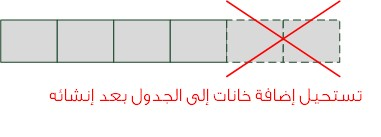
\includegraphics[width=0.7\textwidth]{Chapter_IV-1_Array-add}
\end{figure}

لا تقترح علينا لغة الـ\textenglish{C}
نظاماً آخراً لتخزين البيانات، لكن من الممكن أن ننشئ بأنفسنا هذا النظام بعناصره الكاملة : ستكون الغاية من هذا الفصل و الفصول الموالية اكتشاف حلول لهذا المشكل.

القائمة المتسلسلة هي طريقة لتنظيم سلسلة من البيانات في الذاكرة. هذا يسمح بجمع هياكل
(\textenglish{structures})
مرتبطة ببعضها البعض بواسطة مؤشّرات. يمكننا تمثيلها كالتالي :

\begin{figure}[H]
	\centering
	
\includegraphics[width=0.6\textwidth]{Chapter_IV-1_Linked-list}
\end{figure}

يمكن لكلّ عنصر أن يحتوي على ما نريد : قيمة من نوع 
\InlineCode{int}
أو أكثر،
\InlineCode{double} \dots
بالإضافة إلى ذلك، كلّ عنصر يحتوي على مؤشّر نحو العنصر الموالي :

\begin{figure}[H]
	\centering
	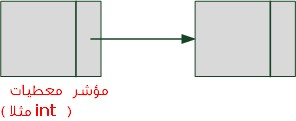
\includegraphics[width=0.5\textwidth]{Chapter_IV-1_Linked-list-data}
\end{figure}

أعرف بأن كلّ هذه المعلومات نظرية و ربّما تبدو لك غير واضحة الآن. احفظ فقط طريقة اتّصال العناصر ببعضها : هي تشكل 
\textbf{سلسلة من المؤشّرات}،
و من هنا نجد الاسم "قائمة متسلسلة". 

\begin{information}
على عكس الجداول، لا تتموضع عناصر القائمة المتسلسلة جنباً إلى جنب في الذاكرة. كل خانة تؤشّر نحو خانة أخرى لا تتواجد ضرورياً بجنب الأخرى.
\end{information}

\section{بناء قائمة متسلسلة}

فلنمرّ الآن إلى صلب الموضوع. سنحاول أن ننشئ بُنية تعمل بنفس المبدأ الذي اكتشفناه الآن.\\
أذكّرك بأن كلّ ما سنقوم به هنا يستدعي تقنيات لغة الـ\textenglish{C}
 التي تعرفها من قبل. لا يوجد شيء جديد، سنكتفي بإنشاء هياكلنا الخاصة و دوال ثم تحويلها إلى نظام منطقي قادر على العمل لوحده.

\subsection{عنصر من القائمة}

من أجل الأمثلة، سننشئ قائمة متسلسلة من أعداد صحيحة. كل عنصر من القائمة له شكل الهيكل التالي :

\begin{Csource}
typedef struct Element Element;
struct Element
{
	int number;
	Element *next;
};
\end{Csource}

\begin{information}
يمكننا أيضاً إنشاء قوائم متسلسلة تحتوي أعدادا عشرية أو حتى جداول أو هياكل. مبدأ القوائم المتسلسلة صالح من أجل أي نوع من البيانات مهما كان، لكن هنا، أنصحك بتبسيط العملية حتى تفهم المبدأ.
\end{information}

قُمنا الآن بإنشاء عنصر واحد من القائمة، يوافق الصورة التي رأيناها أعلاه. على ماذا يحتوي الهيكل ؟

\begin{itemize}
	\item قطعة بيانات، هنا تتمثل في عدد من نوع 
	\InlineCode{int} :
	يمكننا تغيير هذا بأي قطعة أخرى
	(\InlineCode{double}،
	جدول \dots). هذا يعتمد على نوع البيانات التي تريد تخزينها، سيكون عليك تغييرها على حسب حاجتك في البرنامج.
	
	\begin{information}
		إذا أردنا العمل بطريقة عامة، الأمثل هو استعمال مؤشّر نحو الفراغ :
		\InlineCode{void*}.
		هذا يسمح بالتأشير على أي نوع من البيانات.
	\end{information}
	\item مؤشّر نحو عنصر من نفس النوع يسمّى
	\InlineCode{next}.
	هذا ما يسمح بوصل العناصر الواحد بالآخر : كلّ عنصر "يعلم" أين يتواجد العنصر الذي يليه في الذاكرة. كما قلتُ لك مسبقاً، الخانات لا تتواجد جنباً إلى جنب في الذاكرة. هذا هو الاختلاف الكبير بالنسبة للجداول. هذا ما سيمنحنا مرونة أكثر لأنه بإمكاننا بسهولة إضافة خانات أخرى لاحقاً حينما نحتاج إليها.

\begin{information}
	و بالمقابل، لا يمكننا معرفة العنصر السابق، أي أنه من المستحيل الرجوع إلى الخلف انطلاقاً من عنصر من هذا النوع من القوائم. لأننا هنا نتكلّم عن قائمة "بسيطة التسلسل"، بينما توجد قوائم أخرى تسمّى "مزدوجة التسلسل" و تحتوي على مؤشّرات في كلتا الجهتين و بهذا فهي أصعب بقليل.
\end{information}
\end{itemize}


\subsection{هيكل التحكّم}

بالإضافة إلى الهيكل الذي نحن بصدد بنائه (و الذي نضاعفه بعدد المرات التي فيها عناصر أخرى)، سنحتاج إلى هيكل آخر لكي نتحكّم في كامل القائمة المتسلسلة. سيكون لهذا الهيكل الشكل التالي :

\begin{Csource}
typedef struct List List;
struct List
{
	Element *first;
};
\end{Csource}

هذا الهيكل
\InlineCode{List}
يحتوي على مؤشّر نحو أوّل عنصر من القائمة. في الواقع، يجب الاحتفاظ بعنوان العنصر الأول لكي نعرف أين تبدأ القائمة. إذا عرفنا العنصر الأول، يمكننا أن نجد العناصر الأخرى بـ"القفز" من عنصر لآخر بالإستعانة بالمؤشرات الموالية.

\begin{information}
هيكل مكوّن من مركّب واحد هو في الغالب غير مفيد. و مع ذلك، أعتقد أننا سنحتاج أن نضيف إليه لاحقاً مركّبات أخرى، يمكننا مثلاً أن نخزّن به حجم القائمة، أي عدد العناصر التي تحتويها.
\end{information}

لن يكون علينا إنشاء سوى نسخة واحدة من الهيكل
\InlineCode{List}.
هي تسمح بالتحكّم في كلّ القائمة المتسلسلة :
 
\begin{figure}[H]
	\centering
	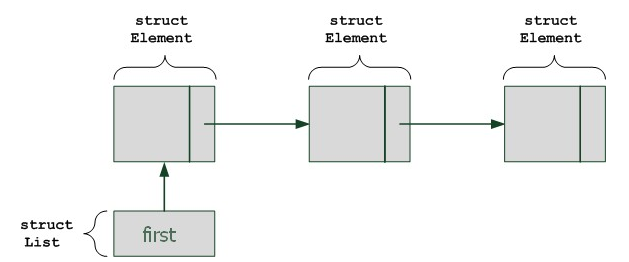
\includegraphics[width=0.9\textwidth]{Chapter_IV-1_List-struct}
\end{figure}

\subsection{آخر عنصر في القائمة}

المخطط أصبح تقريباً كاملاً. ينقصه شيء أخير : نفضّل أن نحفظ العنصر الأخير من القائمة. في الواقع، يجب أن نتوقّف من التقدّم في القائمة المتسلسلة في لحظة ما. كيف سيتسنى لنا أن نقول للبرنامج : "توقف، هذا هو آخر عنصر" ؟

سيكون ممكناً أن نضيف إلى الهيكل 
\InlineCode{List}
مؤشّرا نحو آخر عنصر. لكن هناك ما هو أبسط : يكفي أن يؤشّر آخر عنصر من القائمة على
\InlineCode{NULL}،
أي إعطاء المؤشّر
\InlineCode{next}
القيمة
\InlineCode{NULL}.
هذا سيسمح لنا أخيراً برسم مخطط كامل لبُنية القائمة المتسلسلة :

\begin{figure}[H]
	\centering
	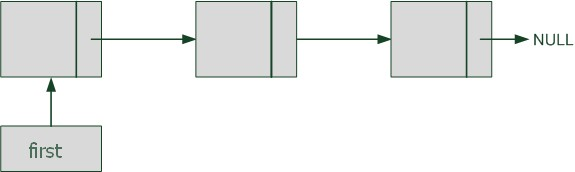
\includegraphics[width=0.8\textwidth]{Chapter_IV-1_List-NULL}
\end{figure}

\section{دوال معالجة القوائم المتسلسلة}

لقد قًمنا بإنشاء هيكلين يسمحان لنا بالتعامل مع القوائم المتسلسلة :

\begin{itemize}
	\item \InlineCode{Element}،
	الذي يوافق عنصراً من القائمة و الذي يمكن لنا أن نكرره بقدر المرات التي نريد.
	\item \InlineCode{List}،
	الذي يتحكّم في مجموع القائمة المتسلسلة. لن نحتاج إلا لنسخة واحدة منه.
\end{itemize}

هذا جيد، لكن ينقص الآن الأهم : الدوال التي ستتعامل مع القائمة المتسلسلة. في الواقع، لن نغيّر "يدويا" محتوى الهياكل في كلّ مرة نحتاج فيها إلى ذلك ! سيكون من الأكثر حكمة و الأكثر نظافة أن نمرّ بدوال تقوم بجعل العمل يتم بشكل تلقائيّ. يجب إنشاؤها هي بدورها.

كنظرة أولى، أقول بأنك نحتاج إلى دوال لكي :

\begin{itemize}
	\item تهيّئ القائمة.
	\item تضيف عنصراً إليها.
	\item تحذف عنصراً منها.
	\item تُظهر محتواها.
	\item تحذف القائمة بأكملها.
\end{itemize}

يمكننا إنشاء دوال أخرى (حساب حجم القائمة مثلاً) لكن يمكن الاستغناء عنها. سنركّز الآن على الدوال التي قمتُ الآن بتعدادها، هذا سيُعطينا قاعدة جيدة. سأدعوك بعد ذلك إلى تحقيق دوال أخرى لكي تتدرّب بعدما تكون قد فهمت المبدأ جيّداً.

\subsection{تهيئة القائمة}

دالة تهيئة القائمة هي أول دالة سنحتاج إلى استدعائها. إذ أنها تقوم بإنشاء هيكل التحكّم و أوّل عنصر من القائمة. أقترح عليك الدالة أسفله و التي سنعلّق عليها بعد ذلك :

\begin{Csource}
List *initialization()
{
	List *list = malloc(sizeof(*list));
	Element *element = malloc(sizeof(*element));
	if (list == NULL || element == NULL)
	{
		exit(EXIT_FAILURE);
	}
	element->number = 0;
	element->next = NULL;
	list->first = element;
	return list;
}
\end{Csource}

نبدأ بإنشاء هيكل التحكّم 
\InlineCode{list}.

\begin{information}
لاحظ أن نوع البيانات هو
\InlineCode{List}
و أن المتغير يسمى
\InlineCode{list}.
تسمح طريقة كتابة الحرف الأول بالتفريق بينهما.
\end{information}

نحجز بطريقة حيّة هيكل التحكّم باستعمال 
\InlineCode{malloc}.
الحجم الذي نحجزه محسوبٌ تلقائياً باستعمال
\InlineCode{sizeof(*list)}.
سيعرف الجهاز بأنه سيحجز المكان الكافي لتخزين الهيكل
\InlineCode{List}.

\begin{information}
 كان بإمكاننا أن نكتُب أيضاً
\InlineCode{sizeof(List)}،
لكن إن أردنا لاحقاً تغيير نوع المؤشّر
\InlineCode{list}
سيكون علينا تحديث الـ\InlineCode{sizeof}
كذلك.
\end{information}

نحجز أيضاً بنفس الطريقة الذاكرة اللازمة لتخزين أول عنصر. نتأكد من أن الحجز الحيّ قد تمّ بنجاح. في حالة خطأ، نوقف البرنامج حالاً باستدعاء الدالة
\InlineCode{exit}.

أما إن تمّ كلّ شيء على ما يُرام، نعرّف قيم أول عنصر من القائمة المتسلسلة :

\begin{itemize}
	\item يتم إعطاء $ 0 $ للمتغير
	\InlineCode{number}
	افتراضياً.
	\item المؤشّر
	\InlineCode{next}
	يؤشّر نحو
	\InlineCode{NULL}
	لأن أول عنصر في القائمة هو أيضاً آخر واحد لحدّ الآن. كما رأينا سابقاً، يجب على آخر عنصر أن يؤشّر نحو
	\InlineCode{NULL}
	ليشير إلى نهاية القائمة.
\end{itemize}

لقد نجحنا الآن في إنشاء قائمة في الذاكرة متكوّنة من عنصر واحد و لها الشكل التالي :

\begin{figure}[H]
	\centering
	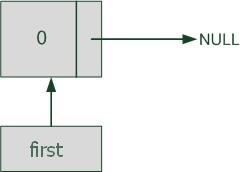
\includegraphics[width=0.3\textwidth]{Chapter_IV-1_List-1-element}
\end{figure}

\subsection{إضافة عنصر}

هنا، تبدأ الأمور في التعقد قليلاً. أين سنضيف عنصراَ جديداً ؟ في بداية القائمة، في نهايتها أو في الوسط ؟

الإجابة هي أنه لدينا الخيار. سنكون أحراراً في اختيار ما نريد. في هذا الفصل، أقترح عليك أن نتعلّم كيفية إضافة عنصر إلى بداية القائمة. من ناحية، هذا الأمر سهل الفهم، و من ناحية أخرى سأعطيك الفرصة في نهاية الفصل في التفكير في طريقة إنشاء دالة تضيف عُنصُراً في مكان محدد من القائمة.

يجدر بنا إنشاء دالة قادرة على أن تضيف عُنصراً جديداً إلى بداية القائمة. و لكي نفهم أكثر، تخيّل أننا في حالة مشابهة لما تعرضه الصورة الموالية : تتكون القائمة من ثلاثة عناصر و نريد أن نضيف لها عُنصراً جديدا في البداية :

\begin{figure}[H]
	\centering
	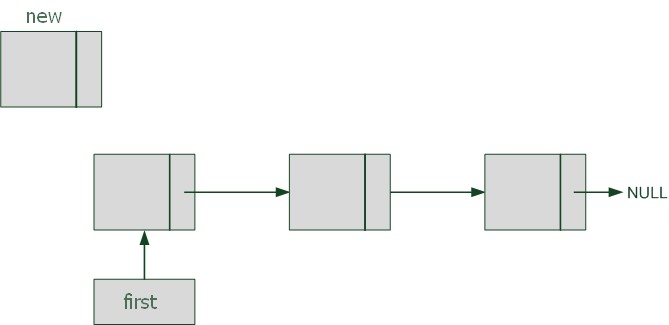
\includegraphics[width=0.8\textwidth]{Chapter_IV-1_List-new}
\end{figure}

يجب أن نقوم بتغيير وضعية المؤشّر
\InlineCode{first}
الخاص بالقائمة و أيضاً المؤشّر
\InlineCode{next}
الخاص بالعنصر الجديد لكي "ندرج" هذا الأخير بشكل صحيح في القائمة. أقترح عليك هذه الشفرة المصدرية التي سنحللها لاحقاً :

\begin{Csource}
void insertion(List *list, int newNumber)
{
	// Creating a new element
	Element *new = malloc(sizeof(*new));
	if (list == NULL || new== NULL)
	{
		exit(EXIT_FAILURE);
	}
	new->number = newNumber;	
	// Inserting the element at the beginning of the list
	new->next = list->first;
	list->first = new;
}
\end{Csource}

تأخذ الدالة
\InlineCode{insertion}
كمعاملات : عنصر التحكّم في القائمة (الذي يحتوي على عنوان أول عنصر) و العدد الذي نريد تخزينه في العنصر الجديد الذي سنقوم بإنشائه. 

سنقوم أولا بحجز المكان اللازم لتخزين العنصر الجديد و نضع به العدد
\InlineCode{newNumber}.
تبقى إذا المرحلة الحساسة : إدراج العنصر الجديد في القائمة المتسلسلة.

لقد اخترنا هنا، تسهيلاً للعملية، إضافة العنصر إلى بداية القائمة. لكي نحدّث المؤشّرات بشكل صحيح، سنعتمد على الخطوتين التاليتين بهذا الترتيب المحدد :

\begin{enumerate}
	\item تأشير العنصر الجديد نحو العنصر الذي سيليه مستقبلاً، أي العنصر الحالي الأول من القائمة.
	\item تأشير المؤشّر
	\InlineCode{first}
	نحو العنصر الجديد.
\end{enumerate}

\begin{warning}
لا يمكننا القيام بهاتين الخطوتين في الترتيب المعاكس ! في الواقع، إن قمنا بجعل المؤشّر
\InlineCode{first}
يؤشّر أولا نحو العنصر الجديد، سنخسر عنوان العنصر الأول من القائمة ! جرّب ذلك، و ستفهم بعد ذلك لمَ عكس الخطوتين أمر مستحيل.
\end{warning}

بإتباع الخطوتين سنتمكن من إدراج العنصر الجديد بشكل صحيح إلى القائمة المتسلسلة :

\begin{figure}[H]
	\centering
	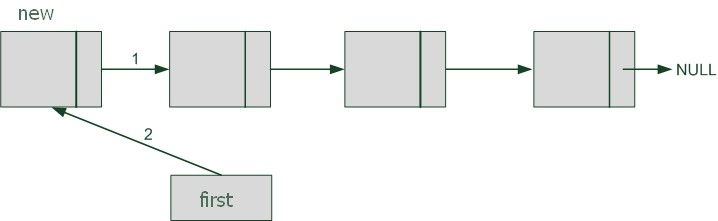
\includegraphics[width=0.9\textwidth]{Chapter_IV-1_List-new-linked}
\end{figure}

\subsection{حذف عنصر}

و نفس الشيء بالنسبة للإضافة، سنركّز الآن على عملية حذف أول عنصر من القائمة. تقنيا، يُسمح بمسح عنصر متواجد في وضعية محددة من وسط القائمة، سيكون هذا واحدا من التمارين التي أقترحها عليك في نهاية الفصل.

عملية حذف عنصر من القائمة المتسلسلة لا تطرح مشكلاً إضافياً. يجب فقط أن نجري التغييرات على المؤشّرات في الترتيب الصحيح لكي لا "نخسر" أية معلومة.

\begin{Csource}
void deletion(List *list)
{
	if (list == NULL)
	{
		exit(EXIT_FAILURE);
	}
	if (list->first != NULL)
	{
		Element *toDelete = list->first;
		list->first = list->first->next;
		free(toDelete);
	}
}
\end{Csource}

نبدأ بالتأكد من أن المؤشّر الذي استقبلناه لا يساوي
\InlineCode{NULL}،
و إلا فلن نتمكّن من العمل. نتأكد بعد ذلك إذا كان هناك على الأقل عنصر واحد في القائمة و إلا فلا يوجد أي شيء لنقوم به.

بعد الانتهاء من هذه الاختبارات، يمكننا حفظ عنوان العنصر الذي نريد حذفه في مؤشّر نسميه
\InlineCode{toDelete}.
يؤشّر بعد ذلك المؤشّر
\InlineCode{first}
نحو العنصر الجديد الأول، و الذي هو حالياً في الوضعية الثانية من القائمة المتسلسلة.

لا يبقى إلا تحرير العنصر الموافق للمؤشّر 
\InlineCode{toDelete}
باستعمال الدالة
\InlineCode{free} :

\begin{figure}[H]
	\centering
	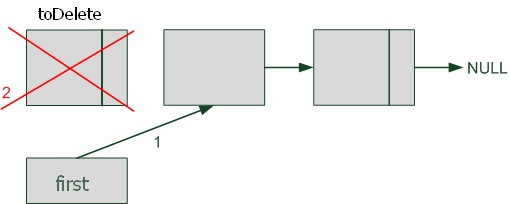
\includegraphics[width=0.7\textwidth]{Chapter_IV-1_List-to-delete}
\end{figure}

هذه الدالة قصيرة لكن هل يمكنك إعادة كتابتها لوحدك ؟ يجب أن نفهم جيداً بأننا يجب أن نقوم بالعمل اتّباعاً لخطوات محددة :

\begin{enumerate}
	\item تأشير
	\InlineCode{first}
	نحو العنصر الثاني.
	\item مسح العنصر الأول باستعمال 
	\InlineCode{free}.
\end{enumerate}

إذا قُمنا بالعكس، سنخسر عنوان العنصر الثاني !

\subsection{إظهار محتوى القائمة المتسلسلة}

لكي نرى بشكل واضح محتوى القائمة المتسلسلة، سيكون من الأمثل أن نكتب دالة عرض ! يكفي أن ننطلق من العنصر الأول و إظهار العناصر واحداً تلو الآخر بـ"القفز" من كتلة لأخرى.

\begin{Csource}
void displayList(List *list)
{
	if (list == NULL)
	{
		exit(EXIT_FAILURE);
	}
	Element *current = list->first;
	while (current != NULL)
	{
		printf("%d -> ", current->number);
		current = current->next;
	}
	printf("NULL\n");
}
\end{Csource}

هذه الدالة بسيطة : ننطلق من العنصر الأول و نُظهر محتوى كلّ عنصر (عدد). نستفيد من المؤشّر 
\InlineCode{next}
لننتقل إلى العنصر المُوالي في كلّ مرة.

يمكننا أن نستمتع بتجريب إنشاء قائمتنا المتسلسلة و إظهارها في الـ\InlineCode{main} :

\begin{Csource}
int main()
{
	List *myList = initialization();
	insertion(myList, 4);
	insertion(myList, 8);
	insertion(myList, 15);
	deletion(myList);
	displayList(myList);
	return 0;
}
\end{Csource}

بالإضافة إلى العنصر الأول (و الذي تركناه هنا يحمل القيمة 0)، نضيف ثلاثة عناصر جديدة لهذه القائمة. ثم نقوم بحذف عنصر واحد. في النهاية، يتم إظهار محتوى القائمة المتسلسلة بالشكل التالي :

\begin{Console}
8 -> 4 -> 0 -> NULL
\end{Console}


\section{اذهب بعيدا}

 لقد قُمنا الآن بكتابة الدوال اللازمة للتحكّم في قائمة متسلسلة : التهيئة، إضافة عنصر، حذف عنصر، إلخ. إليك بعض الدوال التي تنقص و التي أدعوك إلى كتابتها، سيكون هذا بمثابة تمرين جيد لك !

\begin{itemize}
	\item \textbf{إضافة عنصر في وسط القائمة} :
	حالياً، لا يمكننا إضافة عناصر إلا في بداية القائمة، هذا كافٍ بشكل عام. أما إن أردنا إضافة عنصر إلى منتصف القائمة، سيكون علينا أن نكتب دالة تأخذ معاملا إضافيّا : عنوان العنصر الذي يسبق العنصر الجديد في القائمة. ستقوم الدالة بالتقدّم في القائمة إلى حين الوصول إلى العنصر المُراد و تقوم بإضافة العنصر الجديد بعده مباشرة.
	\item \textbf{حذف عنصر من وسط القائمة} :
	المبدأ نفسه بالنسبة للإضافة في وسط القائمة. هذه المرة، يجب عليك أن تضيف معاملا يمثل عنوان العنصر الذي نريد حذفه.
	\item \textbf{تدمير القائمة} :
	يكفي أن نقوم بحذف كل العناصر واحداً تلو الآخر !
	\item \textbf{حجم السلسلة} :
	تشير هذه الدالة إلى كم من عنصر تتكون القائمة المتسلسلة. الأمثل، و في عوض أن يتم حساب هذه القيمة في كلّ مرة، هو أن نضيف عددا صحيحا
	\InlineCode{nbOfElements}
	إلى الهيكل
	\InlineCode{List}.
	يكفي أن نزيد من قيمته في كلّ مرة نضيف فيها عنصراً جديداً للقائمة و أن ننقص من قيمته في كلّ مرة نحذف عنصراً منها.
\end{itemize}

أنصحك بجمع كلّ دوال معالجة القوائم المتسلسلة في ملفين 
\InlineCode{linked\_list.c}
و
\InlineCode{linked\_list.h}
مثلاً. ستكون أوّل مكتبة تكتبها بنفسك ! يمكنك إعادة استعمالها في كلّ برامجك الأخرى التي تحتاج فيها إلى القوائم المتسلسلة.

يمكنك تنزيل مشروع القوائم المتسلسلة الذي يحتوي الدوال التي اكتشفناها سوياً. ستكون هذه بمثابة قاعدة جيدة لك.

\url{http://www.siteduzero.com/uploads/fr/ftp/mateo21/c/listes_chainees.zip}

\section*{ملخّص}

\begin{itemize}
	\item تشكّل القوائم المتسلسلة طريقة جديدة لتخزين البيانات في الذاكرة. هي أكثر مرونة من الجداول لأنها تمكّننا من إضافة و حذف "خانات" في أي لحظة نريد.
	\item لا تحتوي لغة الـ\textenglish{C}
	على نظام تحكّم في القوائم المتسلسلة، إذ يجب أن نكتبه بأنفسنا ! يعتبر هذا طريقة ممتازة للتقدّم في الخوارزميات و البرمجة بشكل عام.
	\item في قائمة متسلسلة، كل عنصر هو عبارة عن هيكل يحتوي عنوان العنصر الموالي.
	\item يُنصح بإنشاء هيكل تحكّم (من نوع
	\InlineCode{List}
	في حالتنا هذه) يحتوي عنوان أول عنصر في القائمة.
	\item توجد نسخة محسّنة - لكن أكثر تعقيداً - من القوائم المتسلسلة و نسمّيها "القوائم مزدوجة التسلسل"، و التي يحتوي كلّ عنصر فيها على عنوان العنصر السابق أيضاً.
\end{itemize}
